\chapter[Calcolo differenziale in più dimensioni]{Calcolo differenziale in più\\dimensioni}
\section{Derivate direzionali}
Dato un versore $\vec v$, con $\vec a+t\vec v$ si indica la retta passante per il punto $\vec a$ e diretta nella direzione di $\vec v$. Con $[\vec a,\vec b]$ si indica invece il segmento delimitato da $\vec a$ e $\vec b$ (inclusi) lungo la retta che passa per i due punti, ossia l'insieme $\{\vec a+t(\vec b-\vec a),\ t\in[0,1]\}$.

Sia $\Omega$ un insieme aperto in $\R^n$, e $f$ una funzione da $\Omega$ a $\R$: poiché $\Omega$ è aperto, possiamo sempre individuare al suo interno un'intorno $B(\vec a,r)\subset\Omega$. Si fissi dunque un versore $\vec v\in\R^n$: muovendosi da $\vec a$ lungo la sua direzione, se $t\in(-r,r)$ allora $\vec a+t\vec v\in\Omega$, perché tale punto è ancora compreso nell'intorno $B(\vec a,r)$. Si restringe allora la $f$ lungo la direzione individuata da $\vec v$, ottenendo la funzione $\phi(t)=f(\vec a+t\vec v)$: essa è definita in $(-r,r)$, e se esiste il limite
\[
\lim_{t\to 0}\frac{\phi(t)-\phi(0)}{t}
\]
esso è la derivata di $\phi$ in $t=0$. Ritornando alla funzione $f$ si ha equivalentemente
\begin{equation} \label{rapporto-incrementale}
\frac{f(\vec a+t\vec v)-f(\vec a)}{t}
\end{equation}
che indica quindi il rapporto incrementale della $f$ ristretta alla direzione di $\vec v$. Si può dare a questo punto la definizione di derivata di $f$ lungo la direzione di $\vec v$.
\begin{definizione} \label{d:derivata-dir}
Si dice \emph{derivata direzionale} della funzione $f\subset\Omega\to\R$ lungo la direzione $\vec v$ in $\vec a\in\Omega$ il limite, quando esiste, del rapporto incrementale:
\[
D_{\vec v}f(\vec a)=\lim_{t\to 0}\frac{f(\vec a+t\vec v)-f(\vec a)}{t}.
\]
\end{definizione}
La restrizione della $f$ lungo $\vec v$ è derivabile, e quindi anche continua. Nel caso in cui $\vec v$ sia uno dei versori della base canonica\footnote{La base canonica di $\R^n$ è composta dagli $n$ vettori $\vec e_j$ in cui la $j$-esima componente è 1, e le altre sono nulle.} di $\R^n$, la derivata direzionale si scrive anche
\[
D_{\vec e_j}f(\vec a)=\drp{f}{x_j}(\vec a),
\]
ed è chiamata \emph{derivata parziale} di $f$ per la direzione $\vec e_j$.
Le derivate direzionali sono ovviamente infinite, mentre le derivate parziali sono tante quante le dimensioni di $\R^n$.
\begin{definizione} \label{d:grad}
Se $f$ ammette tutte le derivate parziali in un punto $\vec a$, si definisce \emph{gradiente} di $f$ in tale punto il vettore
\begin{equation} \label{eq:grad}
\grad f(\vec a)=\bigg(\drp{f}{x_1}(\vec a),\drp{f}{x_2}(\vec a),\dots,\drp{f}{x_n}(\vec a)\bigg).
\end{equation}
\end{definizione}
La derivata parziale è inoltre definita come, ad esempio per $x_1$,
\[
\drp{f}{x_1}(\vec a)=\lim_{t\to 0}\frac{f(\vec a+t\vec e_1)-f(\vec a)}{t}=\lim_{t\to 0}\big[f(a_1+t,a_2,\dots,a_n)-f(a_1,a_2,\dots,a_n)\big]
\]
quindi non è altro che un'operazione di derivazione rispetto soltanto alla variabile $x_1$, mantenendo le rimanenti come costanti. Si possono allora applicare le solite regole di derivazione per le funzioni ad una sola variabile.
\paragraph{Esempi}
\begin{itemize}
\item Sia $f(\vec x)=\scalar{\vec b}{\vec x}$, con $\vec b\in\R^n$. La funzione è per definizione di prodotto scalare equivalente a $f(\vec x)=\sum_{j=1}^nb_jx_j$, quindi chiaramente le derivate parziali esistono tutte e valgono
\[
\drp{f}{x_j}=b_j,
\]
cioè il gradiente di $f$ in $\vec x$ è $\grad f(\vec x)=\vec b$.
\item La funzione $f(\vec x)=\norm{\vec x}$, per definizione, è $f(\vec x)=\sqrt{\sum_{j=1}^nx_j^2}$, quindi le derivate parziali sono per $\vec x\neq\vec 0$
\[
\drp{f}{x_j}=\frac12\left(\sum_{j=1}^nx_j^2\right)^{-\frac{1}{2}}2x_j=x_j\left(\sum_{j=1}^nx_j^2\right)^{-\frac{1}{2}},
\]
quindi il suo gradiente è $\grad f(\vec x)=\dfrac{\vec x}{\norm{\vec x}}$. Si nota anche che $\grad(\norm{\vec x})$ è un versore.
\end{itemize}

Per le funzioni ad una variabile reale, la derivabilità implica automaticamente la continuità. Questo non è più vero in più dimensioni, come mostrato dalla funzione
\[
f(x,y)=\begin{dcases}
\frac{xy^2}{x^2+y^4}	&(x,y)\neq(0,0)\\
0					&(x,y)=(0,0)
\end{dcases}
\]
che è derivabile in $(0,0)$ lungo ogni versore $\vec v=(v_1,v_2)$ ma non è continua in tale punto. Infatti
\[
D_{\vec v}f(0,0)=\lim_{t\to 0}\frac{t^3v_1v_2^2}{t(t^2v_1^2+t^4v_2^4)}=\lim_{t\to 0}\frac{v_1v_2^2}{v_1^2+t^2v_2^4}=
\begin{cases*}
v_2^2/v_1	&se $v_1\neq 0$\\
0			&se $v_1=0$,
\end{cases*}
\]
quindi la derivata esiste per ogni $\vec v$, ma restringendo $f$ al cammino $(t^2,t)$ si ha $f(t^2,t)=1/2$ che è diverso dal valore della funzione in quel punto, quindi non è continua.

Allora la derivabilità in un punto, anche in ogni direzione, di una funzione \emph{non} implica la sua continuità in tale punto. Per garantire la continuità bisogna quindi introdurre un nuovo concetto, quello di differenziabilità.

\section{Differenziabilità}
Per le funzioni da $\R$ a $\R$, la proprietà di derivabilità coincideva in pratica con quella di differenziabilità, ossia della possibilità di scrivere l'incremento della funzione come somma di un termine lineare e di un termine infinitesimo:
\[
f(a+x)=f(a)+\ell x+o(x).
\]
Le due condizioni si implicavano a vicenda, ma questo non accade in più dimensioni: si ha la definizione seguente\footnote{Ovviamente riconducibile al caso di $f\colon\R\to\R$.}.
\begin{definizione} \label{d:differenziabilita}
Sia una funzione $f\colon\Omega\subseteq\R^n\to\R$, con $\Omega$ aperto. Preso un punto $\vec a\in\Omega$, e un $\vec h$ piccolo tale per cui $\vec a+\vec h\in\Omega$, allora $f$ si dice \emph{differenziabile} in $\vec a$ se esiste un'applicazione lineare $L\colon\R^n\to\R$ tale che per $\norm{\vec h}\to 0$ si possibile scrivere
\begin{equation} \label{eq:differenziabilita-app}
f(\vec a+\vec h)-f(\vec a)=L(\vec h)+o(\norm{\vec h}).
\end{equation}
\end{definizione}
L'applicazione $L$ è detta \emph{differenziale primo} di $f$ nel punto $\vec a$, e si indica con $\dd f(\vec a,\cdot)$.
Ogni applicazione lineare da $\R^n$ a $\R$ è rappresentabile % una volta fissata la base, qui quella canonica?
tramite il prodotto interno con un vettore fissato di $\R^n$: allora esiste un vettore $\vlambda\in\R^n$ per cui si può scrivere $L(\vec h)=\scalar{\vlambda}{\vec h}$. Si può dunque formulare la definizione \ref{d:differenziabilita} chiedendo che esista un vettore $\vlambda\in\R^n$ tale per cui
\begin{equation} \label{eq:differenziabilita}
\lim_{\vec h\to\vec 0}\frac{f(\vec a+\vec h)-f(\vec a)-\scalar{\vlambda}{\vec h}}{\norm{\vec h}}=0.
\end{equation}
\begin{osservazione}
Se esiste $\vlambda$ tale per cui valga la \eqref{eq:differenziabilita}, allora è unico.
\end{osservazione}
\begin{proof}
Sia $f$ differenziabile in $\vec a$ per due vettori distinti $\vlambda_1$ e $\vlambda_2$. Si ha allora l'uguaglianza
\[
\scalar{\vlambda_1}{\vec h}+o(\norm{\vec h})=f(\vec a+\vec h)-f(\vec a)=\scalar{\vlambda_2}{\vec h}+o(\norm{\vec h}).
\]
Trascurando il membro centrale si trova che $\scalar{\vlambda_1-\vlambda_2}{\vec h}=o(\norm{\vec h})$. Dividendo per $\norm{\vec h}$, si ottiene $\vec h/\norm{\vec h}$ che è un versore, che sarà indicato con $\vec v$; dunque $\scalar{\vlambda_1-\vlambda_2}{\vec v}=o(1)$, cioè per ogni $\vec v$ si ha che $\scalar{\vlambda_1-\vlambda_2}{\vec v}=0$, dato che l'espressione non dipende da $\norm{\vec h}$. Allora $\vlambda_1-\vlambda_2$ è ortogonale a $\vec v$: poiché l'unico vettore ortogonale ad infiniti vettori (la relazione vale infatti per qualunque $\vec v\in\R^n$) è il vettore nullo, risulta $\vlambda_1=\vlambda_2$.
\end{proof}

La differenziabilità della funzione permette di evitare spacevoli inconvenienti come la discontinuità. Il teorema seguente dimostra la regolarità della funzione differenziabile, oltre a mostrare che $\vlambda$ non è proprio un vettore qualsiasi.
\begin{teorema} \label{t:conseguenze_differenziabilita}
Siano $\Omega$ un aperto di $\R^n$, e la funzione $f\colon\Omega\to\R$. Preso un punto $\vec a\in\Omega$, se $f$ è differenziabile in tale punto allora:
\begin{enumerate}
\item $f$ è continua in $\vec a$;
\item per ogni versore $\vec v\in\R^n$, $f$ ammette le derivate direzionali $D_{\vec v}f(\vec a)$;
\item esiste il gradiente $\grad f(\vec a)$, che è uguale a $\vlambda$;
\item $D_{\vec v}f(\vec a)=\scalar{\grad f(\vec a)}{\vec v}$.
\end{enumerate}
\end{teorema}
\begin{proof}
\begin{enumerate}
\item Poiché $f$ è differenziabile, applicando il modulo alla definizione di differenziabilità si ottiene che $\abs{f(\vec a+\vec h)-f(\vec a)}=\abs{\scalar{\vlambda}{\vec h}+o(\norm{\vec h})}$. L'ultimo membro è maggiorato dalla somma dei moduli dei singoli termini, quindi $\abs{f(\vec a+\vec h)-f(\vec a)}\leq\abs{\scalar{\vlambda}{\vec h}}+o(\norm{\vec h})\leq\norm{\vlambda}\norm{\vec h}+o(\norm{\vec h})$ che tende a 0 se $\vec h$, quindi anche $\norm{\vec h}$, tende a 0. Quindi $f(\vec a+\vec h)\to f(\vec a)$ e la funzione è continua.
\item Fissato un versore $\vec v$, l'incremento lungo la sua direzione è differenziabile come $f(\vec a+t\vec v)-f(\vec a)=\scalar{\vlambda}{t\vec v}+o(\norm{t\vec v})$. Dato che $\norm{t\vec v}=\abs{t}\norm{\vec v}=\abs{t}$, dividendo per $t$ risulta
\[
\frac{f(\vec a+t\vec v)-f(\vec a)}{t}=\scalar{\vlambda}{\vec v}+o(1)\text{, cioè }D_{\vec v}f(\vec a)=\scalar{\vlambda}{\vec v}.
\]
\item Per il secondo punto si ha $D_{\vec v}f(\vec a)=\scalar{\vlambda}{\vec v}$, e quando il versore è della base canonica di $\R^n$, $\vec e_j$, per definizione si ha la derivata parziale, che è quindi
\[
\drp{f}{x_j}(\vec a)=\scalar{\vlambda}{\vec e_j}=\lambda_j\;\then\;\grad f(\vec a)=\vlambda.
\]
\item Quest'ultimo punto segue automaticamente dal fatto che $\grad f(\vec a)=\vlambda$ e $D_{\vec v}f(\vec a)=\scalar{\vlambda}{\vec v}$.\qedhere
\end{enumerate}
\end{proof}
Se $f$ è differenziabile in $\vec a$, allora la mappa $\vec v\mapsto D_{\vec v}f(\vec a)$ è lineare, in quanto le derivate direzionali sono una combinazione lineare di $\vec v$, cioè
\[
D_{\vec v}f(\vec a)=\scalar{\grad f(\vec a)}{\vec v}=\sum_{i=1}^n\drp{f}{x_i}(\vec a)v_i.
\]
Inoltre, noto il gradiente della funzione, lo si può sostituire nella \eqref{eq:differenziabilita} e se il limite è vero, cioè se esiste finito
\[
\lim_{\vec x\to\vec a}\frac{f(\vec x)-f(\vec a)-\scalar{\grad f(\vec a)}{\vec x,\vec a}}{\norm{\vec x-\vec a}}
\]
allora la funzione è differenziabile.

\begin{definizione} \label{d:grafico-iperpiano}
Data una funzione $f\colon\Omega\subseteq\R^n\to\R$, l'insieme
\[
\Gamma=\big\{(\underbracket[.5pt]{x_1,x_2,\dots,x_n}_{\vec x},x_{n+1}),\ \vec x\in\Omega,\ x_{n+1}=f(\vec x)\big\}\subset\R^{n+1}
\]
è il \emph{grafico} di $f$.

In un punto $\vec a\in\Omega$, si definisce \emph{iperpiano tangente} al grafico di $f$ in $\big(\vec a,f(\vec a)\big)$ l'insieme dei punti di $\R^{n+1}$ tali per cui $x_{n+1}=f(\vec a)+\scalar{\grad f(\vec a)}{\vec x-\vec a}$.
\end{definizione}
\begin{osservazione}
Se $f$ è differenziabile in $\vec a$, si ha che $D_{\vec v}f(\vec a)=\scalar{\grad f(\vec a)}{\vec v}$, quindi
\[
\abs{D_{\vec v}f(\vec a)}\leq\norm{\grad f(\vec a)};
\]
il gradiente quindi maggiora le derivate direzionali. La massima crescita, o pendenza, del grafico della $f$ si ha allora nella direzione del gradiente, per la quale la disuguaglianza sopra è un'uguaglianza. Il vettore gradiente indica allora la massima pendenza di $f$.
\end{osservazione}
Nel caso di una funzione vettoriale, $\vec f\colon\R^n\to\R^m$, non si fa altro che generalizzare nelle $m$ componenti di $\vec f$ quanto detto precedentemente: la derivata direzionale non è unica ma ce n'è una per ogni componente della funzione, ed è quindi una funzione sempre vettoriale in $\R^m$, definita nel generico punto $\vec a$ come il limite, quando esiste,
\[
D_{\vec v}\vec f(\vec a)=\lim_{t\to 0}\frac{\vec f(\vec a+t\vec v)-\vec f(\vec a)}{t}=\big(D_{\vec v}f_1(\vec a),D_{\vec v}f_2(\vec a),\dots,D_{\vec v}f_m(\vec a)\big).
\]
Le derivate parziali seguono la stessa regola delle funzioni scalari, semplicemente ogni funzione può ammettere al più $m$ derivate parziali in ogni variabile, quindi non più $n$ ma $mn$ derivate.
Se esistono tutte le derivate parziali in $\vec a$, si raccolgono tutte in una matrice $m\times n$
\[
\begin{bmatrix}
\drp{f_1}{x_1}	&\drp{f_1}{x_2}	&\cdots	&\drp{f_1}{x_n}\\
\drp{f_2}{x_1}	&\drp{f_2}{x_2}	&\cdots	&\drp{f_2}{x_n}\\
\vdots			&\vdots			&\ddots	&\vdots\\
\drp{f_m}{x_1}	&\drp{f_m}{x_2}	&\cdots	&\drp{f_1}{x_n}
\end{bmatrix}\qquad\qquad(\jac\vec f)_{ij}=\drp{f_i}{x_j},
\]
detta \emph{jacobiana} di $\vec f$. Per le funzioni scalari, che hanno una sola componente, la jacobiana è composta soltanto della prima riga e si riduce quindi al gradiente. Ogni riga della jacobiana, in effetti, è il gradiente di una singola componente. Se la funzione è in una sola variabile la jacobiana diventa un vettore, e sarà indicata più semplicemente con $\vec f'(\vec a)$.

La definizione di differenziabilità ricalca quella già data nella \ref{d:differenziabilita} per le funzioni scalari, con ovviamente $m$ dimensioni al posto di una soltanto.
\begin{definizione}
La funzione $\vec f\colon\Omega\subset\R^n\to\R^m$ si dice differenziabile nel punto $\vec a\in\Omega$ se e solo se esiste un'applicazione lineare $L\colon\R^n\to\R^m$ tale per cui si può scrivere
\begin{equation} \label{eq:differenziabilita-app-vett}
\vec f(\vec a+\vec h)=\vec f(\vec a)+L(\vec h)+\vec o(\vec h).
\end{equation}
\end{definizione}
Quindi $\vec f$ è differenziabile in $\vec a$ se e solo se lo sono tutte le sue componenti $f_1,f_2,\dots,f_m$.
A questa applicazione $L$ %vedere se bisogna fissare una base prima di associarla ad una matrice!
si può associare una matrice, fissata, $\Lambda\in\mat_{m,n}(\R)$, cioè con $m$ righe e $n$ colonne, tale che $L(\vec h)=\Lambda\vec h$. Si riscrive dunque la definizione precedente questa volta richiedendo che esista una tale matrice $\Lambda$ per cui valga
\begin{equation} \label{eq:differenziabilita-vett}
\lim_{\vec h\to\vec 0}\frac{\vec f(\vec a+\vec h)-\vec f(\vec a)-\Lambda\vec h}{\norm{\vec h}}=0.
\end{equation}

In maniera del tutto simile al teorema \ref{t:conseguenze_differenziabilita}, dalla differenziabilità delle funzioni vettoriali discendono alcune proprietà importanti:
\begin{enumerate}
\item $\vec f$ è continua in $\vec a$;
\item esistono tutte le derivate direzionali $D_{\vec v}\vec f(\vec a)$, per qualunque versore $\vec v\in\R^n$;
\item la matrice per cui vale la \eqref{eq:differenziabilita-vett} è $\Lambda=\jac\vec f(\vec a)$;
\item $D_{\vec v}\vec f(\vec a)=\jac\vec f(\vec a)\vec v$.
\end{enumerate}
Inoltre le generiche derivate direzionali si ottengono dall'equazione
\[
D_{\vec v}\vec f(\vec a)=\jac\vec f(\vec a)\vec v=\sum_{i=1}^m\bigg(\sum_{j=1}^n\drp{f_i}{x_j}(\vec a)v_j\bigg)\vec e_i,
\]
dove $\{\vec e_k\}$ sono i vettori della base canonica di $\R^m$.
Anche in questo caso $L$ è chiamata differenziale primo, e si identifica con la jacobiana:
\[
\dd\vec f(\vec a;\cdot)\colon\vec h\mapsto\jac\vec f(\vec a)\vec h.
\]
\begin{teorema}[del differenziale totale]
Siano $\Omega$ un aperto in $\R^n$, $\vec a$ un suo punto e la funzione $f\colon\Omega\to\R$. Se esiste un intorno $B(\vec a,r)\subset\Omega$ per cui esistono tutte le $n$ derivate parziali di $f$, e sono tutte continue nel punto $\vec a$, allora $f$ è differenziabile in $\vec a$.
\end{teorema}
Nel caso di $\R^2$ si dà la seguente dimostrazione, generalizzabile eventualmente per $\R^n$ con $n$ qualunque.
\begin{proof}
Siano $\vec x=(x,y)\in B(\vec a,r)$ e $\vec a=(a_1,a_2)$. Si dimostra che
\begin{equation} \label{eq:difftot}
\frac{f(x,y)-f(a_1,a_2)-\scalar{\grad f(\vec a)}{\vec x-\vec a}}{\norm{\vec x-\vec a}}\to 0,
\end{equation}
in modo che $f$ sia differenziabile in $\vec a$.

Si può calcolare $f(x,y)-f(a_1,a_2)$ come $f(x,y)-f(a_1,y)+f(a_1,y)-f(a_1,a_2)$. I primi due termini corrispondono all'incremento di $f$ fissato $y$ (quindi lungo la direzione di $x$), mentre i secondi due all'incremento fissato $a_1$ (quindi lungo $y$). Il risultato è ancora ovviamente un punto interno a $\Omega$ (figura \ref{fig:differenziale_totale}).
\begin{figure}
	\tikzsetnextfilename{differenziale-totale}
	\centering
	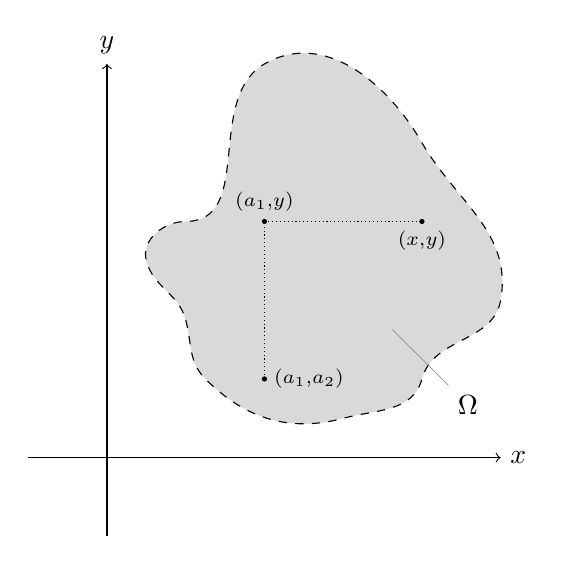
\begin{tikzpicture}
		\draw [black,->] (-1,0) -- (5,0) node[right]{$x$};
		\draw [black,->] (0,-1) -- (0,5) node[above]{$y$};
		\draw [fill=black!15!white,dashed] (1,1.75) to[out=-75,in=135] (1.25,1) to[out=-45,in=195] (3,.5) to[out=15,in=-105] (4,1) to[out=75,in=-100] (5,2) to[out=80,in=-60] (4,4) to[out=120,in=30] (2,5) to[out=210,in=0] (1,3) to[out=180,in=105] (.5,2.5) to[out=-75,in=105] (1,1.75);
		\node [pin={[pin distance=1cm]-45:{$\Omega$}}] at (3.5,1.75) {};
		\draw [densely dotted] (2,1) node[right]{$\scriptstyle(a_1,a_2)$} to (2,3) node[above]{$\scriptstyle(a_1,y)$};
		\draw [densely dotted] (2,3) -- (4,3) node[below]{$\scriptstyle(x,y)$};
		\node [fill=black,circle,scale=.2] at (2,1) {};
		\node [fill=black,circle,scale=.2] at (2,3) {};
		\node [fill=black,circle,scale=.2] at (4,3) {};
	\end{tikzpicture}
	\caption{Incremento $\vec x-\vec a$ scomposto nelle due direzioni lungo gli assi cartesiani in $\R^2$.}
	\label{fig:differenziale_totale}
\end{figure}

Applicando il teorema di Lagrange a $f(\cdot,y)$ e $f(a_1,\cdot)$, che sono entrambe derivabili per ipotesi, dato che corrispondono alle derivate parziali rispettivamente in $x$ e $y$, si ottiene che
\[
f(x,y)-f(a_1,y)=(x-a_1)\drp{f}{x}(\xi,y)\qeq f(a_1,y)-f(a_1,a_2)=(y-a_2)\drp{f}{y}(a_1,\eta)
\]
per qualche $(\xi,y)$ e $(a_1,\eta)$ in $\Omega$.
Il numeratore della \eqref{eq:difftot} si riscrive quindi come
\begin{align*}
&(x-a_1)\drp{f}{x}(\xi,y)+(y-a_2)\drp{f}{y}(a_1,\eta)-\bigg[(x-a_1)\drp{f}{x}(a_1,a_2)+(y-a_2)\drp{f}{y}(a_1,a_2)\bigg]=\\
=&(x-a_1)\bigg[\drp{f}{x}(\xi,y)-\drp{f}{x}(a_1,a_2)\bigg]+(y-a_2)\bigg[\drp{f}{y}(a_1,\eta)-\drp{f}{y}(a_1,a_2)\bigg],
\end{align*}
il cui modulo è minore della somma dei moduli dei termini, quindi
\begin{align*}
\leq&\abs{x-a_1}\abs{\drp{f}{x}(\xi,y)-\drp{f}{x}(a_1,a_2)}+\abs{y-a_2}\abs{\drp{f}{y}(a_1,\eta)-\drp{f}{y}(a_1,a_2)}\leq\\
\leq&\norm{\vec x-\vec a}\abs{\drp{f}{x}(\xi,y)-\drp{f}{x}(a_1,a_2)}+\norm{\vec x-\vec a}\abs{\drp{f}{y}(a_1,\eta)-\drp{f}{y}(a_1,a_2)}=\\
\leq&\norm{\vec x-\vec a}\left[\abs{\drp{f}{x}(\xi,y)-\drp{f}{x}(a_1,a_2)}+\abs{\drp{f}{y}(a_1,\eta)-\drp{f}{y}(a_1,a_2)}\right].
\end{align*}
Allora la \eqref{eq:difftot} è maggiorata dal termine tra parentesi quadre. Per $\vec x\to\vec a$ si ha $(\xi,y)\to\vec a$ e anche $(a_1,\eta)\to\vec a$, e poiché le derivate parziali per ipotesi sono continue risulta che la \eqref{eq:difftot} tende a 0, quindi la $f$ è differenziabile in $\vec a$.
\end{proof}
Se $f$ è una funzione vettoriale da $\R^n$ a $\R^m$, il teorema richiede che tutte le derivate parziali $\frac{\ddp f_i}{\ddp x_j}$ con $1\leq i\leq m$ e $1\leq j\leq n$ siano continue in $\vec a$.

\begin{definizione}
Sia $\Omega$ un aperto di $\R^n$ e $f\colon\Omega\to\R$: si dice che $f\in\cont{1}(\Omega)$ se in ogni punto di $\Omega$ esistono e sono continue tutte le derivate parziali di $f$.
\end{definizione}
\begin{corollario}
Se una funzione appartiene alla classe $\cont{1}(\Omega)$, allora è differenziabile in tutto $\Omega$.
\end{corollario}
La dimostrazione segue immediatamente dal teorema precedente.

\section{Differenziazione di funzioni composte}
\begin{teorema}
Sia $\Omega$ un insieme aperto in $\R^n$, $\vec a\in\Omega$ e $\vec f\in\Omega\to\R^m$ differenziabile in $\vec a$; sia quindi $\vec g\in\R^m\to\R^p$ differenziabile in $\vec b=\vec f(\vec a)$.
Allora la funzione composta $\vec h=\vec g\circ\vec f\colon\R^n\to\R^p$ è differenziabile in $\vec a$, e vale la relazione
\begin{equation} \label{eq:composizione_differenziali}
\dd\vec h(\vec a;\cdot)=\dd\vec g(\vec b;\cdot)\circ\dd\vec f(\vec a;\cdot)=\dd\vec g\big(\vec b;\dd\vec f(\vec a;\cdot)\big),
\end{equation}
vale a dire che la jacobiana di $\vec h$ in $\vec a$ è il prodotto ordinato della jacobiana di $\vec g$ per quella di $\vec f$:
\[
\jac\vec h(\vec a)=\jac\vec g\big(\vec f(\vec a)\big)\jac\vec f(\vec a).
\]
Il prodotto tra queste matrici è possibile, dato che sono rispettivamente $p\times m$ e $m\times n$, e si ottiene quindi che la jacobiana di $\vec h$ ha $p$ righe e $n$ colonne. Il prodotto \emph{non} è commutativo, in quanto non è nemmeno possibile eseguirlo scambiando l'ordine dei fattori, diversamente dal caso di funzioni da $\R$ in $\R$.
\end{teorema}
Sviluppando il prodotto tra le due matrici si ha che la componente della jacobiana di $\vec h$ è, con $1\leq i\leq p$ e $1\leq j\leq n$,
\[
\big(\!\jac\vec h(\vec a)\big)_{ij}=\drp{h_i}{x_j}(\vec a)=\sum_{k=1}^m\drp{g_i}{y_k}\big(\vec f(\vec a)\big)\drp{f_k}{x_j}(\vec a),
\]
dove $y_k$ è la variabile relativa a $\vec g$, ossia $y_k=f_k(\vec a)$.
\begin{teorema}[di Lagrange] \label{t:lagrange_piu_variabili}
Sia $\Omega$ un aperto di $\R^n$, $\vec a$ e $\vec b$ due punti interni ad esso tali che $[\vec a,\vec b]\subset\Omega$, e $g\colon\Omega\to\R$ una funzione differenziabile in tutto $\Omega$. Allora esiste un punto $\vxi\in[\vec a,\vec b]$ per il quale $g(\vec b)-g(\vec a)=\scalar{\grad g(\vxi)}{\vec b-\vec a}$.
\end{teorema}
\begin{proof}
Sul segmento $\vec b-\vec a$ si costruisce una funzione vettoriale $\vec f(t)=\vec a+t(\vec b-\vec a)$, con $t\in[0,1]$\footnote{Dato che tale segmento è interno ad $\Omega$, anche ``sporgendo'' un poco oltre gli estremi si resterà sempre nell'insieme, quindi volendo si può limitare $t$ anche a $(-\epsilon,1+\epsilon)$}: componendola con $g$ si ottiene che $(g\circ\vec f)(t)=g[\vec a+t(\vec b-\vec a)]$, tale che $g\circ\vec f\colon[0,1]\to\R$ e le si applica il teorema \ref{t:lagrange} di Lagrange per funzioni reali a variabili reali nell'intervallo $[0,1]$, ottenendo che esiste $\theta\in(0,1)$ tale per cui $(g\circ\vec f)(1)-(g\circ\vec f)(0)=(g\circ\vec f)'(\theta)$, cioè
\[
g(\vec b)-g(\vec a)=\jac g\big(\vec f(\theta)\big)\jac\vec f=\scalar{\grad g\big(\vec f(\theta)\big)}{\vec b-\vec a}.
\]
Il punto $\vec f(\theta)$ è il punto $\vxi$ cercato della tesi.
\end{proof}
Si potrebbe formulare una versione di questo teorema anche per le funzioni vettoriali, per il quale al posto del gradiente in $\vec a$ si avrebbe la jacobiana in $\vec a$: si applicherebbe semplicemente il teorema di Lagrange appena dimostrato per ognuna delle componenti di $\vec g$. In realtà un tale teorema non ha ragione di esistere, come mostra il seguente controesempio. Sia $\vec g(t)=(\cos t,\sin t)$, con $\vec a=0$ e $\vec b=2\pi$. Una versione vettoriale del teorema di Lagrange porterebbe a concludere che esisterebbe $x\in(0,2\pi)$ per cui
\[
\vec g(2\pi)-\vec g(0)=\begin{pmatrix}\grad g_1\\\grad g_2\end{pmatrix} 2\pi=\begin{pmatrix}-\sin x\\\cos x\end{pmatrix} 2\pi= \begin{pmatrix}1\\0\end{pmatrix}-\begin{pmatrix}1\\0\end{pmatrix}= \begin{pmatrix}0\\0\end{pmatrix},
\]
ossia $\sin x=0$ e $\cos x=0$ contemporaneamente, chiaramente assurdo.

Il problema sta nel fatto che sebbene sia realmente possibile applicare il teorema \ref{t:lagrange_piu_variabili} alle varie componenti di una funzione vettoriale, non si può affermare che sia soddisfatto per ognuna in un unico punto: ogni componente soddisfa il teorema in punti diversi.
\begin{teorema}[dell'incremento finito]
Sia $\Omega\in\R^m$ un aperto e $\vec g\colon\Omega\to\R^p$ differenziabile in $[\vec a,\vec b]\subset\Omega$. Allora esiste $c\geq 0$ tale per cui $\norm{\vec g(\vec b)-\vec g(\vec a)}\leq c\norm{\vec b-\vec a}$.
\end{teorema}
Un ``buon'' valore di questa quantità $c$ è ad esempio
\[
c=\sqrt{mp}\max_{\substack{1\leq i\leq p\\1\leq j\leq m}}\sup_{\vec x\in[\vec a,\vec b]}\abs{\drp{g_i}{x_j}(\vec x)}.
\]
Se tutte le derivate parziali sono nulle, si ha $c=0$ quindi la funzione è costante.

\section{Diffeomorfismi}
\begin{definizione} \label{d:diffeomorfismo}
Siano $A\in\R^n$ e $B\in\R^n$ due insiemi aperti. Una funzione $\vec f\colon A\to B$ biiettiva si dice \emph{diffeomorfismo} di $A$ su $B$ se $\vec f$ è differenziabile e la sua inversa $\vec f^{-1}\colon B\to A$ è anch'essa differenziabile.
\end{definizione}
Anche l'inverso di un diffeomorfismo è ovviamente, a sua volta, un diffeomorfismo: in questa classe di funzioni si trovano in particolare i cambiamenti di coordinate, che infatti per queste proprietà si possono applicare senza problemi di irregolarità nelle funzioni.
\begin{teorema}
Sia $\vec f\colon A\to B$ con $A\in\R^n$ e $B\in\R^m$. Se risulta che:
\begin{itemize}
	\item $\vec f$ è differenziabile $\forall\vec x\in A$;
	\item ?
	\item $\det\jac\vec f(\vec x)$ per ogni $\vec x\in A$,
\end{itemize}
allora $\vec f$ è un diffeomorfismo.
\end{teorema}
Le traslazioni sono dei diffeomorfismi: sia ad esempio in $\R^3$ la funzione $\vec T(\vec x)=\vec x+\vec b$, essa è indubbiamente differenziabile, e lo è anche la sua inversa $\vec T^{-1}(\vec x)=\vec x-\vec b$.
Calcolando le matrici jacobiane di queste funzioni si ha
\[
\jac\vec T(\vec x)=\jac\vec T^{-1}(\vec x)=\begin{bmatrix}
1&0&0\\0&1&0\\0&0&1
\end{bmatrix}
\]
per ogni $\vec x\in\R^3$, generalizzabile ovviamente a qualunque dimensione.
Si nota che il prodotto delle due jacobiane dà la matrice identità $3\times 3$: questo non è dovuto al fatto che entrambe le jacobiane sono già di per sé matrici identità, ma è un risultato generale per tutti i diffeomorfismi. Se infatti si compongono una funzione $\vec f$ con la sua inversa $\vec f^{-1}$, si ottiene l'identità $\vec f^{-1}\circ\vec f=\textup{id}_A$ sull'insieme $A$; calcolando le jacobiane,
\[
\jac(\vec f^{-1}\circ\vec f)(\vec x)=\jac\vec f^{-1}\big(\vec f(\vec x)\big)\jac \vec f(\vec x)=\jac\vec x=I_n,
\]
che è la jacobiana della funzione identità, per ogni $\vec x\in A$. Di conseguenza, passando ai determinanti si trova che $\det\jac \vec f(\vec x)\neq 0$, e che essa è l'inversa di $\jac\vec f^{-1}\big(\vec f(\vec x)\big)$.

Tra i diffeomorfismi più importanti si trovano i cambiamenti di coordinate, come quello in coordinate polari: esso è una trasformazione biunivoca tra $\R^2$ privato dell'origine e $(0,\pinf)\times[0,2\pi)$, che porta la coppia di coordinate cartesiane $(x,y)$ nella coppia $(\rho,\theta)$, che indica rispettivamente la distanza dall'origine degli assi e l'angolo che la retta congiungente l'origine e il punto formerebbe con il semiasse positivo delle ascisse, con le trasformazioni
\begin{equation}
\begin{cases}
\rho=\sqrt{x^2+y^2}\\
x=\rho\cos\theta\\
y=\rho\sin\theta
\end{cases}.
\end{equation}

Sia $\vec T\colon(0,\pinf)\times[0,2\pi)\to\R^2\setminus\{(0,0)\}$ definita come $\vec T\colon(\rho,\theta)\mapsto(\rho\cos\theta,\rho\sin\theta)\equiv(x,y)$: il determinante della jacobiana della trasformazione è sempre non nullo, infatti
\[
\det\jac\vec T(\rho,\theta)=
	\begin{vmatrix}
	\cos\theta	&-\rho\sin\theta\\
	\sin\theta	&\rho\cos\theta
	\end{vmatrix}
=\rho(\cos^2\theta+\sin^2\theta)=\rho\neq 0
\]
essendo definito in $(0,\pinf)$, quindi è un diffeomorfismo.
Posta $f$ una funzione qualunque da $\R^2\setminus\{(0,0)\}$ a $\R$ (per semplicità), si può comporre con $\vec T$ ottenendo
\[
g(\rho,\theta)=f\big(\vec T(\rho,\theta)\big).
\]
Si ricava $f(x,y)$ invertendo il processo:
\[
f(x,y)=g\big(\vec T^{-1}(x,y)\big).
\]
Calcolando le jacobiane, risulta allora per la $g$
\begin{equation} \label{eq:composizione_jacobiane_polari1}
\jac g(\rho,\theta)=\jac f\big(\vec T(\rho,\theta)\big)\jac\vec T(\rho,\theta)
\end{equation}
mentre per la $f$ si ha
\begin{multline} \label{eq:composizione_jacobiane_polari2}
\jac f(x,y)=\jac g\big(\vec T^{-1}(x,y)\big)\jac\vec T^{-1}(x,y)=\\
=\jac g\big(\vec T^{-1}(x,y)\big)\big[\jac\vec T\big(\vec T^{-1}(x,y)\big)\big]^{-1}=\jac g\big(\vec T^{-1}(x,y)\big)\big[\jac\vec T(\rho,\theta)\big]^{-1},
\end{multline}
sfruttando il fatto che $\jac\vec T\big(\vec T^{-1}(x,y)\big)\equiv\jac\vec T(\rho,\theta)$ è l'inversa di $\jac\vec T^{-1}(x,y)$, come visto in precedenza.

Dalle \eqref{eq:composizione_jacobiane_polari1} e \eqref{eq:composizione_jacobiane_polari2} si possono dunque calcolare le formule per la derivazione in coordinate polari: esse sono
\begin{equation} \label{eq:jacobiane_polari}
\begin{gathered}
\grad g(\rho,\theta)
=\grad f(x,y)
	\begin{pmatrix}
	\cos\theta	&-\rho\sin\theta\\
	\sin\theta	&\rho\cos\theta
	\end{pmatrix}\\
\grad f(x,y)
=\grad g(\rho,\theta)
	\begin{pmatrix}
	\cos\theta			&\sin\theta\\
	-\frac{\sin\theta}{\rho}	&\frac{\cos\theta}{\rho}
	\end{pmatrix}
=\bigg(\drp{g}{\rho},\drp{g}{\theta}\bigg)
	\begin{pmatrix}
	\frac{x}{\sqrt{x^2+y^2}}	&\frac{y}{\sqrt{x^2+y^2}}\\
	-\frac{y}{x^2+y^2}		&\frac{x}{x^2+y^2}.
	\end{pmatrix},
\end{gathered}
\end{equation}
dunque le derivate della funzione dopo la trasformazione in coordinate polari sono
\begin{equation} \label{eq:derivate_polari}
\begin{gathered}
\drp{g}{\rho}=\cos\theta\,\drp{f}{x}+\sin\theta\,\drp{f}{y}\\
\drp{g}{\theta}=-\rho\sin\theta\,\drp{f}{x}+\rho\cos\theta\,\drp{f}{y}.
\end{gathered}
\end{equation}

\section{Derivate seconde}
Sia $f$ una funzione scalare definita da un aperto $\Omega\subset\R^n$ a $\R$, e si supponga che per ogni $\vec x\in\Omega$ esista la derivata $D_{\vec v}f(\vec x)$, lungo la direzione indicata dal versore $\vec v$. Fissato un altro versore $\vec w$, se esiste la derivata di questa derivata lungo $\vec w$ in un punto $\vec a$, ossia $D_{\vec w}\big(D_{\vec v}f(\vec a)\big)$, che equivale al limite
\[
\lim_{t\to 0}\frac{D_{\vec v}f(\vec a+t\vec w)-D_{\vec v}f(\vec a)}{t},
\]
allora si dice che $f$ è due volte derivabile in $\vec a$ lungo le direzioni $\vec v$ e $\vec w$, \emph{rigorosamente nell'ordine} rappresentato. Tale derivata seconda si scrive come $D^2_{\vec v,\vec w}f(\vec a)$, indicando nei pedici i due versori, nell'ordine della prima e della seconda derivata.
Se inoltre i versori appartengono alla base canonica di $\R^n$, allora la derivata si scrive anche come
\[
D^2_{\vec e_i,\vec e_j}f(\vec a)=\frac{\ddp^2f}{\ddp x_i\ddp x_j}(\vec a).
\]
Le derivate parziali seconde con versori differenti si dicono miste.

Se esistono tutte le derivate seconde parziali in $\vec a$ di $f$ (in tutto sono $n^2$) allora esse formano, in ordine, una matrice quadrata $n\times n$, detta \emph{matrice hessiana} di $f$ in $\vec a$ (da valutare nel punto):
\[
\hes f=\begin{bmatrix}
\dfrac{\ddp^2f}{\ddp x_1^2}		&\dfrac{\ddp^2f}{\ddp x_1\ddp x_2}	&\cdots 	&\dfrac{\ddp^2f}{\ddp x_1\ddp x_n}\\
\dfrac{\ddp^2f}{\ddp x_2\ddp x_1}	&\dfrac{\ddp^2f}{\ddp x_2^2}		&\cdots 	&\dfrac{\ddp^2f}{\ddp x_2\ddp x_n}\\
\vdots 							&\vdots 							&\ddots 	&\vdots\\
\dfrac{\ddp^2f}{\ddp x_n\ddp x_1}	&\dfrac{\ddp^2f}{\ddp x_n\ddp x_2}	&\cdots 	&\dfrac{\ddp^2f}{\ddp x_n^2}
\end{bmatrix}\qquad\qquad(\hes f)_{ij}=\dfrac{\ddp^2f}{\ddp x_i\ddp x_j}.
\]
L'hessiana di fatto rappresenta la jacobiana del gradiente come vettore riga.

L'ordine di derivazione è importante non solo per il risultato dell'operazione, ma anche per l'esistenza stessa del risultato, come dimostrano i seguenti esempi in $\R^2$:
\begin{itemize}
\item Sia $f(x,y)=x^2y^{1/3}$. Le derivate prime parziali nell'origine sono entrambe nulle, altrimenti
\[
\drp{f}{x}(x,y)=2x\sqrt[3]{y}\qeq\drp{f}{y}(x,y)=\begin{dcases*}\nexists&in $(x,0)$ con $x\neq 0$\\\frac{x^2}{3y^{2/3}}&altrove\end{dcases*}.
\]
Nell'origine, la derivata seconda rispetto a $y$ e poi a $x$, nell'ordine, ossia $\frac{\ddp}{\ddp x}\big(\frac{\ddp f}{\ddp y}\big)(0,0)$, non esiste, mentre la derivata seconda rispetto a $x,y$ è
\[
\frac{\partial^2f}{\partial x\partial y}(x,y)=\drp{}{y}\bigg(\drp{f}{x}\bigg)(0,0)=\lim_{y\to 0}\frac{\frac{\ddp f}{\ddp x}(0,y)-\frac{\ddp f}{\ddp x}(0,0)}{y}=0.
\]
\item Sia $f$ definita come
\[
f(x,y)=\begin{dcases*}0&in $(0,0)$\\\frac{xy^3}{x^2+y^2}&altrove\end{dcases*}.
\]
Nell'origine si ha $\grad f(0,0)=(0,0)$, altrimenti il gradiente di $f$ è
\[
\grad f(x,y)=\bigg(\frac{y^5-x^2y^3}{(x^2+y^2)^2},\frac{3x^3y^2+xy^4}{(x^2+y^2)^2}\bigg).
\]

Allora si ha
\begin{align*}
&\frac{\ddp^2f}{\ddp y\ddp x}=\lim_{x\to 0}\frac{\frac{\ddp f}{\ddp y}(x,0)-\frac{\ddp f}{\ddp y}(0,0)}{x}=\lim_{x\to 0}\frac0{x}=0,\\
%in che punti???
&\frac{\ddp^2f}{\ddp x\ddp y}=\lim_{y\to 0}\frac{\frac{\ddp f}{\ddp x}(0,y)-\frac{\ddp f}{\ddp x}(0,0)}{y}=\lim_{y\to 0}\frac{y}{y}=1.
\end{align*}
\end{itemize}
Per certe funzioni, però, le derivate seconde non dipendono dall'ordine di derivazione, come spiegato dal seguente teorema.
\begin{teorema}[di Schwartz] \label{t:schwarz}
Siano $\Omega$ un aperto di $\R^n$, $\vec a$ un punto interno ad esso, $\vec v$ e $\vec w$ due versori di $\R^n$ e $f$ una funzione definita da $\Omega$ a $\R$. Se esiste un intorno di $\vec a$ contenuto in $\Omega$ in cui esistono sia $D^2_{\vec v,\vec w}f$ che $D^2_{\vec w,\vec v}f$ e sono continue in $\vec a$, allora esse coincidono in tale punto.
\end{teorema}
\begin{corollario}
Se la funzione $f$ è di classe $\cont{2}(\Omega)$, cioè esistono e sono continue tutte le derivate parziali prime e seconde in $\Omega$, allora le derivate miste coincidono; vale a dire, la matrice hessiana è simmetrica.
\end{corollario}
Se la funzione poi è vettoriale, la matrice hessiana avrà dei vettori come componenti, e il teorema di Schwarz vale ancora componente per componente.%?

Quando $f\colon\Omega\to\R$ è differenziabile in ogni punto $\vec x\in\Omega$, il suo differenziale primo $\dd f(\vec x;\cdot)$ è una funzione da $\R^n$ a $\R$ lineare, definita come $\dd f(\vec x;\vec h)=\scalar{\grad f(\vec x)}{\vec h}$, $\forall\vec h$ tale che l'incremento $\vec x+\vec h$ appartenga ancora ad $\Omega$. Fissato però l'incremento $\vec h$, si può considerare $\dd f(\cdot;\vec h)=\scalar{\grad f(\cdot)}{\vec h}$ che è una funzione di variabile $\vec x\in\Omega$ a valori reali, proprio come $f$. Se questa funzione\footnote{Poiché le derivate parziali sono $n$ e non una sola, in realtà il differenziale primo come $\dd f(\cdot;\vec h)$ rappresenta più di una funzione: è la combinazione lineare delle derivate parziali.} $\dd f(\cdot;\vec h)$ è differenziabile in un punto $\vec a$ di $\Omega$, allora si dice che $f$ è due volte differenziabile in $\vec a$.

Alcune condizioni implicano o sono implicate dal fatto che $f$ è due volte differenziabile in $\vec a$:
\begin{enumerate}
\item (\textit{necessaria e sufficiente}) ogni derivata parziale prima è differenziabile in $\vec a$;
\item (\textit{necessaria}) esistono tutte le derivate parziali seconde in $\vec a$, e quelle miste coincidono\footnote{Questa affermazione non equivale al teorema \ref{t:schwarz} di Schwarz, in quanto le ipotesi sono differenti.};
\item (\textit{necessaria}) ogni derivata direzionale prima è differenziabile in $\vec a$, quindi esistono tutte le derivate seconde direzionali indipendentemente dell'ordine (per il punto precedente) e si ha
\[
D^2_{\vec v,\vec w}f(\vec a)=\sum_{i,j=1}^n\frac{\ddp^2f}{\ddp x_i\ddp x_j}(\vec a)v_iw_j,
\]
la quale è chiamata \emph{forma quadratica} di $f$ in $\vec a$;
\item (\textit{sufficiente}) in un intorno di $\vec a$ esistono e sono continue tutte le derivate prime parziali, ed esistono tutte le derivate seconde parziali e sono continue in $\vec a$;
\item (\textit{sufficiente}) $f$ è di classe $\cont{2}(\Omega)$.
\end{enumerate}

\section{Formula di Taylor}
Sia $f\colon\Omega\to\R$, con $\Omega\subseteq\R^n$ e $\vec a\in\Omega$. La $f$ si dice $k$-volte differenziabile in $\vec a$ se esiste il $(k-1)$-esimo differenziale della funzione nel punto.
La generica derivata parziale $k$-esima di $f$ si può allora scrivere come
\[
\frac{\partial^kf}{\partial x_1^{j_1}\dots\partial x_n^{j_n}},
\]
con $0\leq j_1,\dots,j_n\leq n$ e $\sum_{i=1}^nj_i=k$; gli indici $j_i$ indicano quante volte si sta derivando $f$ rispetto alla $i$-esima componente.
Per comodità si può eventualmente usare una notazione multiindice $\vec j=(j_i,\dots,j_n)$, con $\vec j\in\N^n$.

Sia quindi $f$ una funzione differenziabile $k$ volte in $\vec a$: si costruisce la mappa
\begin{equation} \label{eq:diff-kesimo}
\dd^kf(\vec a;\cdot;\dots;\cdot)\colon\underbracket[.5pt]{\R^n\times\dots\times\R^n}_\text{$k$ volte}\to\R,
\end{equation}
che è lineare in ogni variabile e tale per cui
\begin{equation}
\dd^kf(\vec a;\vec h^{(1)};\dots;\vec h^{(k)})=
\sum_{i_1,\dots,i_k}^n\frac{\partial^kf}{\partial x_{i_1}\dots\partial x_{i_n}}
h_{i_1}^{(1)}\dots h_{i_n}^{(k)}.
\end{equation}
Questa formula è utile nel caso in cui $\vec h^{(1)}=\dots=\vec h^{(k)}=\vec h\in\R^n$, per il quale si impiega un unico vettore per l'incremento per tutte le componenti: per snellire la notazione allora si scrive più semplicemente
\[
\dd^kf(\vec a;\underbracket[.5pt]{\vec h;\dots;\vec h}_\text{$k$ volte})=\dd^kf(\vec a;\vec h).
\]
Con questa notazione si può scrivere dunque
\begin{equation}
\dd^kf(\vec a;\vec h)=\sum\frac{\partial^kf}{\partial x_1^{j_1}\dots\partial x_n^{j_n}} h_1^{j_1}\dots h_n^{j_n},
\end{equation}
ancora con $0\leq j_1,\dots,\leq k$ e $\sum_{i=1}^n=k$, dove $k$ è l'ordine del differenziale. Il differenziale di ordina $k$ è quindi%? quindi cosa, che non si capisce un cazzo
 composto da una somma di monomi ciascuno di grado $k$, cioè è un polinomio omogeneo di grado $k$, nelle componenti del vettore $\vec h$.

Per come è composto il differenziale si ha quindi che sostituendo all'incremento fissato $\vec h$ un incremento variabile lungo la stessa direzione, ossia $t\vec h$, risulta
\begin{equation}
\dd^kf(\vec a;t\vec h)=t^k\dd^kf(\vec a;\vec h).
\end{equation}
Dividendo il differenziale per $\norm{\vec h}^k$ si ottiene dunque un polinomio omogeneo di grado nullo, e costante quando valutato sulle semirette con origine sull'origine degli assi\footnote{Non è corretto affermare che sia costante valutato sulle \emph{rette} passanti per l'origine, poiché per $\vec h=\vec 0$ la funzione non è definita, dato che il denominatore è nullo.}, infatti
\[
\frac{\dd^kf(\vec a;t\vec h)}{\norm{t\vec h}^k}=\frac{t^k\dd^kf(\vec a;\vec h)}{\abs{t}^k\norm{\vec h}^k}=\frac{\dd^kf(\vec a;\vec h)}{\norm{\vec h}^k}
\]
che è indipendente da $t$ quindi costante su tutta la semiretta.

Siano ora $\vec w\neq\vec 0$ e $f\in\cont{k}(\Omega)$. Per $t$ sufficientemente piccolo, $\vec a+\vec w\in\Omega$, quindi la funzione $F(t)\defeq f(\vec a+t\vec w)$ è di classe $\cont{k}$ in un intorno di $t=0$, dove è assicurato che sia composta da due funzioni una, $f$, di classe $\cont{k}$ per definizione, e l'altra, $\vec a+t\vec w$, di classe $\cont{\infty}$. Al di fuori di $\mathcal U(0)$ non è più certo che $\vec a+t\vec w$ appartenga ancora a $\Omega$, al di fuori del quale $f\notin\cont{k}$. Dunque la $F$ è una funzione definita da $\mathcal U(0)$ a $\R$. Nel centro $t=0$ si può dunque sviluppare in serie di Taylor fino all'ordine $k$: le sue derivate sono
\begin{equation}\begin{aligned}
F'(t)	&=\scalar{\grad f(\vec a+t\vec w)}{\vec w}=\sum_{j=1}^n\drp{f}{x_j}(\vec a+t\vec w)w_j=\dd f(\vec a+t\vec w;\vec w)\\
F''(t)	&=\sum_{j=1}^nw_j\bigg[\sum_{i=1}^n\drp{}{x_i}\Big(\drp{f}{x_j}(\vec a+t\vec w)w_i\Big)\bigg]=\\
		&=\sum_{i,j=1}^n\frac{\partial^2f}{\partial x_i\partial x_j}(\vec a+t\vec w)w_iw_j=\\
		&=\vec w^t\hes f(\vec a+t\vec w)\vec w=\dd^2f(\vec a+t\vec w;\vec w),
\end{aligned}\end{equation}
e così via per induzione %ma dove???
si ha $F^{(n)}(t)=\dd^nf(\vec a+t\vec w;\vec w)$, per ogni $0\leq n\leq k$.
Operando il cambio di variabile $\vec x\defeq\vec a+\vec w$ (con il segmento $[\vec a,\vec x]\subset\Omega$) lo sviluppo di Taylor di $F$ con resto di Lagrange, centrato in $t=0$, nell'intervallo $[0,1]$ è
\[
F(1)=\frac1{0!}F(0)1^0+\frac1{1!}F'(0)1^1+\frac1{2!}F''(0)1^2+\dots+\frac1{(k-1)!}F^{(k-1)}(0)1^{k-1}+\frac1{k!}F^{(k)}(\theta)
\]
per qualche $\theta\in(0,1)$. Per la definizione di $F$ quindi risulta, dato che $F(1)=f(\vec x)$, che
\begin{multline} \label{eq:formula_taylor_lagrange_piu_variabili}
f(\vec x)=f(\vec a)+\dd f(\vec a;\vec x-\vec a)+\frac1{2!}\dd^2f(\vec a;\vec x-\vec a)+\dots\\
\dots+\frac1{(k-1)!}\dd^{k-1}f(\vec a;\vec x-\vec a)+\frac1{k!}\dd^kf(\vxi;\vec x-\vec a)
\end{multline}
dove $\vxi\in(\vec a,\vec x)$, corrispondente al punto $\theta$ precedente.

Con il resto di Peano, invece, si ha, sempre all'ordine $k$,
\begin{equation} \label{eq:formula_taylor_peano_piu_variabili}
f(\vec x)=\sum_{j=0}^k\frac1{j!}\dd^jf(\vec a;\vec x-\vec a)+o(\norm{\vec x-\vec a}^k).
\end{equation}

\section{Estremanti liberi}
\begin{definizione}
Sia $f\colon\Omega\to\R$ dove $\Omega\in\R^n$ e sia $\vec a\in\Omega$. Il punto $\vec a$ si dice punto di estremo locale per $f$ in $\Omega$, e in particolare:
\begin{itemize}
\item \emph{punto di massimo locale} se $\exists B(\vec a,r)\subset\Omega$ in cui $f(\vec a)\geq f(\vec x)$, per ogni $\vec x\in B(\vec a,r)$;
\item \emph{punto di minimo locale} se $\exists B(\vec a,r)\subset\Omega$ in cui $f(\vec a)\leq f(\vec x)$, per ogni $\vec x\in B(\vec a,r)$.
\end{itemize}
\end{definizione}
Il massimo o il minimo locale sono il valore assunto dalla funzione nel rispettivo punto estremante. Il massimo è assoluto se la definizione è estendibile a tutto l'insieme $\Omega$, cioè se $f(\vec a)\geq f(\vec x)$ per ogni $\vec x\in\Omega$; analogamente per i minimi.
Infine, il punto estremante si dice \emph{forte} se l'uguaglianza si ha solo in $\vec a$ e non anche altrove.

Si ricorda il teorema di Weierstra\ss\ \ref{t:weierstrass} che afferma che se $f$ è continua in $E$ compatto, allora essa ha massimo e minimo assoluti in $E$. Individuato questo insieme compatto, gli estremi (locali) possono trovarsi in $\mathring{E}$ o in $\partial E$: in questi casi si dicono, rispettivamente, estremi \emph{liberi} ed estremi \emph{vincolati}. Se individuare gli estremi vincolati in una sola dimensione consisteva al più nell'analisi di due soli punti, in più dimensioni la frontiera di un insieme è solitamente costituita da infiniti punti: occorrono quindi metodi diversi per i due casi.
Di seguito ci si occuperà soltanto degli estremi liberi.

\begin{teorema}[di Fermat]
Sia $f\colon\Omega\to\R$, con $\Omega\in\R^n$ aperto, differenziabile in $\vec a\in\Omega$. Se $\vec a$ è un punto estremante per $f$, allora $\grad f(\vec a)=\vec 0$.
\end{teorema}
\begin{proof}
Si consideri l'incremento della $f$ lungo la direzione data dal versore $\vec e_i$ della base canonica
\[
g_i(t)=f(\vec a+t\vec e_i).
\]
Sia ora $\vec a$ un punto di massimo: allora $f(\vec a)\geq f(\vec a+t\vec e_i)$ per ogni $t$ opportunamente contenuto in un intervallo $(-\delta,\delta)$ tale che $f$ sia ancora differenziabile in $\vec a\pm\delta\vec e_i$, quindi per cui $g_i$ è derivabile in $(-\delta,\delta)$.
Dunque si ha $g_i(t)-g_i(0)\leq 0$, sia per $-\delta<t<0$ che per $0<t<\delta$; dividendo entrambi gli incrementi per $t$ e passando al limite rispettivamente per $t\to0^\mp$, si ottiene la derivata sinistra e destra di $g_i$ in $0$, che per il teorema di permanenza del segno sono rispettivamente non negativa e non positiva. Poiché $g$ è derivabile in $0$, le derivate devono coincidere e non può che risultare
\[
\lim_{t\to 0^-}g_i(t)=\lim_{t\to 0^+}g_i(t)=g_i'(0)=\drp{f}{x_i}(\vec a)=0,
\]
questo naturalmente per ogni $i\in\{1,\dots,n\}$, cioè tutte le derivate parziali di $f$ sono nulle in $\vec a$: allora $\grad f(\vec a)=\vec 0$.
\end{proof}
Ovviamente la condizione data è soltanto sufficiente, come mostra la funzione $f(x)=x^2-y^2$, che nell'origine ha gradiente nullo ma tale punto non è un estremante; i punti stazionari non estremanti si dicono \emph{punti di sella}. In ogni caso, è necessaria soltanto per i punti estremanti \emph{liberi}, dato che $\Omega$ è aperto, e in cui $f$ è differenziabile. Rimangono esclusi quindi i punti in cui $f$ non è differenziabile, da analizzare singolarmente, e gli estremi vincolati.

Sia $f\in\cont{2}(\Omega)$. In $\vec a$, punto estremante locale di $f$, il gradiente è nullo: per $\vec h\to\vec 0$, arbitrariamente piccolo e tale per cui $\vec a+\vec h\in\Omega$, per il teorema di Taylor con resto di Peano risulta
\begin{align}
&f(\vec a+\vec h)=f(\vec a)+\scalar{\grad f(\vec a)}{\vec h}+\frac12\dd^2f(\vec a;\vec h)+o(\norm{\vec h}^2)\\
&f(\vec a+\vec h)-f(\vec a)=\frac12\dd^2f(\vec a;\vec h)+o(\norm{\vec h}^2).
\end{align}
Sfruttando l'uguaglianza %da dimostrare!
$\dd^2f(\vec a;\vec h)=\vec h^t\hes f(\vec a)\vec h$, e in seguito raccogliendo $\norm{\vec h}^2$ si ottiene l'equazione
\begin{equation}
f(\vec a+\vec h)-f(\vec a)=\frac12\norm{\vec h}^2\left[\frac{\vec h^t\hes f(\vec a)\vec h}{\norm{\vec h}^2}+o(1)\right].
\end{equation}
Il segno del secondo membro, che sarà quindi il segno dell'incremento della funzione da $\vec a$ a $\vec a+\vec h$, è quindi determinato dalla forma quadratica $\vec h^t\hes f(\vec a)\vec h$. Si $F(\vec h)$ la funzione definita come
\[
F(\vec h)=\frac{\vec h^t\hes f(\vec a)\vec h}{\norm{\vec h}^2}.
\]
Essa è una funzione omogenea di grado 0, quindi è costante sulle semirette con origine nell'origine degli assi\footnote{Le forme quadratiche sono polinomi omogenei di grado 2, quindi dividendole per una norma al quadrato, anch'essa di grado 2, si ottiene un polinomio di grado nullo.}: infatti fissato $\vec v$ e per $t>0$ si ha
\[
F(t\vec v)=\frac{(t\vec v)^t\hes f(\vec a)(t\vec v)}{\norm{t\vec v}^2}=\frac{t^2}{\abs{t}^2}\frac{\vec v^t\hes f(\vec a)\vec v}{\norm{\vec v}^2}=F(\vec v).
\]
La $F$ è dunque definita in $\R^n\setminus\{\vec 0\}$, è continua e differenziabile dove definita, e costante quando ristretta alle rette passanti per l'origine. Si possono allora analizzare i valori assunti da $F$ su una superficie sferica qualsiasi centrata nell'origine, ad esempio fissando $\norm{\vec h}=1$. Questa superficie, che corrisponde poi a $\partial B(\vec 0,1)$, è chiusa e limitata, cioè è un insieme compatto. Per il teorema di Weierstra\ss\ dunque la $F$ ammette un minimo e un massimo assoluto $m,M$ in $\partial B(\vec 0,1)$, cioè esistono $\vec u,\vec w\neq\vec 0$ tali per cui
\begin{equation} \label{eq:maxmin_quadratica}
m=F(\vec u)\leq F(\vec h)\leq F(\vec w)=M.
\end{equation}
Per il teorema di Fermat, allora, si ha $\grad f(\vec u)=\grad f(\vec w)=\vec 0$.
Nel caso in cui $mM\neq 0$ risulta:
\begin{itemize}
\item se $0<m\leq M$, $F$ assume soltanto valori tra $m$ e $M$ che sono entrambi positivi, quindi $F(\vec h)>0$ e per $\norm{\vec h}$ sufficientemente piccolo il termine $o(\norm{\vec h}^2)$ non influisce sul segno, quindi si ha $f(\vec a+\vec h)-f(\vec a)>0$ cioè $\vec a$ è un punto di minimo locale;
\item analogamente se $m\leq M<0$, $\vec a$ è un punto di massimo locale;
\item se $m<0<M$, la $F$ cambia di segno, quindi $\vec a$ è un punto di sella.
\end{itemize}
Quando invece $mM=0$, il segno è determinato da $o(\norm{\vec h}^2)$, quindi questo metodo non porta ad alcun risultato.
Rimane quindi da trovare il segno di $m$ e $M$. Poiché $f$ è differenziabile due volte, la sua matrice hessiana è simmetrica, e come già visto si può rappresentare (fissata la base, cioè quella canonica) la forma quadratica che è il differenziale secondo con l'espressione $\vec h^t\hes f(\vec a)\vec h$. Sia quindi $q(\vec x)=\vec x^t\hes f(\vec a)\vec x$: si ha che $F(\vec x)=q(\vec x)/\norm{\vec x}^2$, e vale ancora la \eqref{eq:maxmin_quadratica}.
Le derivate parziali di $F$ sono
\[
\drp{}{x_k}\norm{\vec x}^2=\drp{}{x_k}\left(\sum_{i=1}^nx_i^2\right)=2x_k,
\]
e
\[\begin{split}
\drp{q}{x_k}(\vec x)	&=\drp{}{x_k}\left(\sum_{i,j=1}^n\big(\hes f(\vec a)\big)_{ij}x_ix_j\right)=\\
					&=\sum_{i,j=1}^n\big(\hes f(\vec a)\big)_{ij}(\delta_{ik}x_j+\delta_{jk}x_i)=\\
					&=\sum_{j=1}^n\big(\hes f(\vec a)\big)_{kj}x_j+\sum_{i=1}^n\big(\hes f(\vec a)\big)_{ik}x_i=\\
					&=\sum_{j=1}^n\big(\hes f(\vec a)\big)_{kj}x_j+\sum_{i=1}^n\big(\hes f(\vec a)\big)_{ki}x_i=\\
					&=2\sum_{j=1}^n\big(\hes f(\vec a)\big)_{kj}x_j=\\
					&=2\big(\hes f(\vec a)\vec x\big)_j,
\end{split}\]
dove si è potuto cambiare gli indici dell'hessiana da $ik$ a $ki$ poiché è simmetrica.
Allora risulta
\[\begin{split}
\drp{F}{x_k}(\vec x)	&=\norm{\vec x}^{-4}\left[\norm{\vec x}^2\drp{q}{x_k}(\vec x)-q(\vec x)\drp{}{x_k}\norm{\vec x}^2\right]=\\
					&=\norm{\vec x}^{-4}\left[\norm{\vec x}^22\big(\hes f(\vec a)\vec x\big)_k-q(\vec x)2x_k\right],
\end{split}\]
dunque
\begin{equation}
\begin{split}
\grad F(\vec x)	&=2\norm{\vec x}^{-4}\big[\norm{\vec x}^2\hes f(\vec a)\vec x-q(\vec x)\vec x\big]=\\
				&=\frac2{\norm{\vec x}^2}\left[\hes f(\vec a)\vec x-\frac{q(\vec x)\vec x}{\norm{\vec x}^2}\right].
\end{split}
\end{equation}
Nei punti $\vec u$ e $\vec v$ estremanti di $F$ si ha dunque $\grad F(\vec x)=\vec 0$, quindi dato che $\vec x$ non è nullo si ha
\begin{equation}
\hes f(\vec a)\vec x=\frac{q(\vec x)}{\norm{\vec x}^2}\vec x=F(\vec x)\vec x,
\end{equation}
cioè $F(\vec x)$ è un autovalore di $\hes f(\vec a)$ a cui è associato proprio l'autovettore $\vec x$. Gli autovalori della matrice hessiana sono tanti quanti la dimensione di $\R^n$, e poiché è simmetrica, sono tutti reali.
Di conseguenza il massimo autovalore di $\hes f(\vec a)$ è anche il massimo di $F(\vec x)$, e lo stesso per il minimo: individuando gli autovalori dell'hessiana in $\vec a$ si trova quindi la natura del punto estremante.
La forma quadratica $q(\vec x)=\vec x^t\hes f(\vec a)\vec x$ si dice
\begin{itemize}
\item\emph{definita positiva} se $q(\vec x)>0$, che significa $0<m\leq M$;
\item\emph{semidefinita positiva} se $q(\vec x)\geq 0$, cioè esiste $\vec v\neq\vec 0$ per cui $q(\vec v)=0$, e questo corrisponde a $0\leq m\leq M$;
\item\emph{indefinita} se esistono $\vec y,\vec z$ tali che $q(\vec y)<0<q(\vec z)$, cioè $m<0<M$;
\item\emph{semidefinita negativa} se $q(\vec x)\leq 0$, cioè $m\leq M\leq 0$;
\item\emph{definita negativa} se $q(\vec x)<0$, che significa $m\leq M<0$,
\end{itemize}
ovviamente per $\vec x\neq\vec 0$ in cui $q(\vec x)=0$ in ogni caso.
Si giunge quindi ai seguenti risultati:
\begin{itemize}
\item se $m>0$, $\vec a$ è un punto di minimo locale forte;
\item se $M<0$, $\vec a$ è un punto di massimo locale forte;
\item se $m<0<M$, $\vec a$ è un punto di sella;
\item se $\vec a$ è un punto di minimo locale (qualsiasi), $q(\vec x)$ è semidefinita positiva;
\item se $\vec a$ è un punto di massimo locale (qualsiasi), $q(\vec x)$ è semidefinita negativa.
\end{itemize}
Se $f$ è una funzione a due sole variabili, ha due autovalori per quanto detto in precedenza: il polinomio caratteristico dell'hessiana è
\begin{equation}\begin{split}
P(\lambda)=\det(\hes f(\vec a)-\lambda I_n)	&=\begin{vmatrix}f_{xx}(\vec a)-\lambda&f_{xy}(\vec a)\\f_{xy}(\vec a)&f_{yy}(\vec a)-\lambda\end{vmatrix}=\\
										&=\lambda^2-(f_{xx}-f_{yy})\lambda+(f_{xx}f_{yy}-f_{xy}^2)=\\
										&=\lambda^2-\big(\tr\hes f(\vec a)\big)\lambda+\det\hes f(\vec a).
\end{split}\end{equation}
Poiché è utile ai fini di conoscere la natura del punto estremante solo sapere il segno degli autovalori, cioè delle due radici del polinomio, e dato che $P(\lambda)=(\lambda-m)(\lambda-M)$, si ha che $m+M=\tr\hes f(\vec a)$ e $mM=\det\hes f(\vec a)$, quindi:
\begin{itemize}
\item se $\det\hes f(\vec a)=0$, non si può affermare niente;
\item se $\det\hes f(\vec a)>0$, si passa considerare la somma delle radici, perciò
	\begin{itemize}
	\item se $\tr\hes f(\vec a)>0$, $\vec a$ è un punto di minimo;
	\item se $\tr\hes f(\vec a)<0$, $\vec a$ è un punto di massimo;
	\end{itemize}
\item se $\det\hes f(\vec a)<0$, $m$ e $M$ sono discordi quindi $\vec a$ è un punto di sella.
\end{itemize}
Infine se $\det\hes f(\vec a)>0$, certamente $f_{xx}$ e $f_{yy}$ sono concordi, altrimenti $f_{xx}f_{yy}-f_{xy}^2$ non potrà mai essere positivo: allora anziché calcolare la traccia della matrice hessiana si può ulteriormente semplificare, guardando soltanto il segno di $f_{xx}$.
